\input{../YKY-preamble.tex}
\setmainfont[BoldFont=AlibabaSans-Regular.otf]{AlibabaSans-Light.otf}

\usepackage[active,tightpage]{preview}		% for continuous page(s)
\renewcommand{\PreviewBorder}{0.5cm}
\renewcommand{\thempfootnote}{\arabic{mpfootnote}}

\usepackage[absolute,overlay]{textpos}		% for page number on upper left corner

\usepackage{color}
\usepackage{mathtools}
\usepackage[hyperfootnotes=false]{hyperref}

% \usepackage[backend=biber,style=numeric]{biblatex}
% \bibliography{../AGI-book}
% \renewcommand*{\bibfont}{\footnotesize}

\usetikzlibrary{shapes}
\usepackage[export]{adjustbox}				% ??
\usepackage{bm}
\usepackage{verbatim} % for comments
% \usepackage{newtxtext,newtxmath}	% Times New Roman font

% \numberwithin{equation}{subsection}

\newcommand{\underdash}[1]{%
	\tikz[baseline=(toUnderline.base)]{
		\node[inner sep=1pt,outer sep=10pt] (toUnderline) {#1};
		\draw[dashed] ([yshift=-0pt]toUnderline.south west) -- ([yshift=-0pt]toUnderline.south east);
	}%
}%

% Tic-Tac-Toe symbols
% \newcommand{\bO}[0]{\raisebox{-0.2em}{\textbf{O}}}
% \newcommand{\Xb}[0]{\raisebox{-0.2em}{\textbf{X}}}

%\DeclareSymbolFont{symbolsC}{U}{txsyc}{m}{n}
%\DeclareMathSymbol{\strictif}{\mathrel}{symbolsC}{74}
\DeclareSymbolFont{AMSb}{U}{msb}{m}{n}
\DeclareSymbolFontAlphabet{\mathbb}{AMSb}
% \setmathfont{Latin Modern Math}

% \newcommand{\highlight}[1]{\colorbox{pink}{$\displaystyle #1$}}

% \newcommand{\emp}[1]{{\color{violet}\textbf{#1}}}
\let\oldtextbf\textbf
\renewcommand{\textbf}[1]{\textcolor{blue}{\oldtextbf{#1}}}

\newcommand*\confoundFace{$\vcenter{\hbox{\includegraphics[scale=0.2]{../2020/../confounded-face.jpg}}}$}
\newcommand{\underconst}{\includegraphics[scale=0.5]{../2020/UnderConst.png}}
\newcommand{\KBsymbol}{\vcenter{\hbox{\includegraphics[scale=1]{../KB-symbol.png}}}}
\newcommand{\witness}{\scalebox{0.6}{$\blacksquare$}}
% \newcommand{\Heytingarrow}{\mathrel{-}\mathrel{\triangleright}}
% \providecommand\Heytingarrow{\relbar\joinrel\mathrel{\vcenter{\hbox{\scalebox{0.75}{$\rhd$}}}}}

\begin{document}

\begin{preview}

\cc{
\title{\vspace{-2.2cm} \bfseries\color{blue}{\large 逻辑化 AGI 基础}}
}{
\title{\vspace{-2.2cm} \bfseries\color{blue}{\large Logicalized AGI basics}}
}

% \author{YKY} % Your name
\date{\vspace{-3.2cm}} % Date, can be changed to a custom date

\maketitle

\setcounter{section}{-1}

% (1) Circled page number on upper left corner
\begin{textblock*}{5cm}(2.1cm,2.3cm) % {block width} (coords) 
{\color{red}{\large \textcircled{\small 1}}}
\end{textblock*}

\begin{minipage}{\textwidth}
\setlength{\parskip}{0.4\baselineskip}

\cc{
这是 \textbf{强化学习} 最基本的 setup}{
This is our basic \textbf{RL} (reinforcement learning) setup}\footnote{The above diagram is somewhat inaccurate as there are subtle differences between the notions of "state" and Working Memory.  In RL, state usually refers to the external environment  through observations.  WM is slightly different in the sense that an internal belief may be \textit{wrong} about the environment --- eg, mistaking seeing something that doesn't exist.  There is on-going research as to the relation between RL and WM.  I have not fully resolved this issue.
	\begin{equation}
	\vcenter{\hbox{\includegraphics[scale=0.5]{../2021/RL-WM-architecture.png}}}
	\end{equation}
	\vspace{-0.7cm}}:
\begin{equation}
\vcenter{\hbox{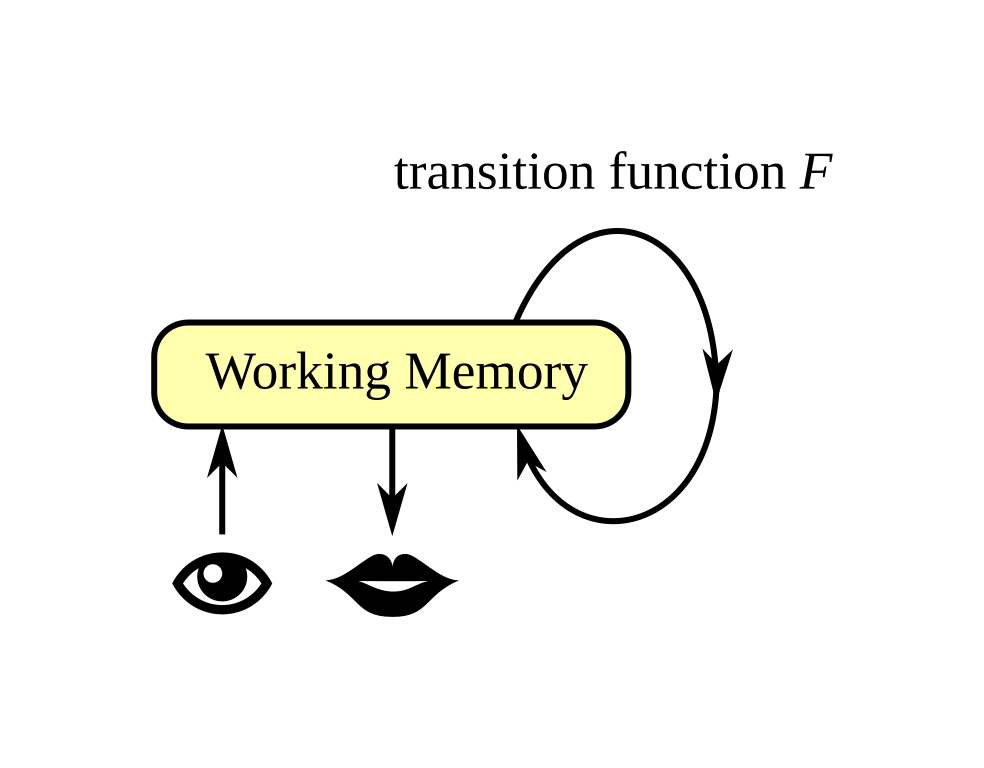
\includegraphics[scale=0.7]{../2021/minimal-RL-architecture.png}}}
\end{equation}
\cc{
	状态转移函数 $F$ 负责 \textbf{更新} 工作记忆 (\textbf{WM}). 如果 $F$ 在一个 \textbf{闭环} 内训练,它似乎可以 ``\textbf{解释}'' (或 预测) 输入的讯息。
}{
\textbf{WM} (working memory) is \textbf{updated} by a transition function.  If this transition function is trained in a \textbf{closed loop}, it may be able to "explain" (in the sense of predicting) the input data.	
}

In classical logic-based AI, \textbf{inductive learning} means searching for a \textbf{theory} $T$ (= set of logic rules) that ``explains'' or \textbf{implies} positive examples but not negative ones:
\begin{equation}
\mbox{\large\(
T \vdash e^{+}, \quad T \nvdash e^{-}
\)}
\end{equation}
While logic learning is powerful, it relies on \textbf{combinatorial search} and was too inefficient, which caused ``AI Winter''.

\cc{
我理论的重点是: 透过 $F$ 在 RL 闭环内的训练,可以做到 \textbf{发现} 逻辑理论 $T$ 的效果。 }{
The main thrust of my argument is that training the function $F$ in the RL closed loop can effectively \textbf{discover} the logic theory $T$.}
\end{minipage}
\end{preview}

\begin{preview}
\begin{minipage}{\textwidth}
\setlength{\parskip}{0.4\baselineskip}	

\begin{textblock*}{20cm}(2.1cm,2cm) % {block width} (coords) 
	{\color{red}{\large \textcircled{\small 2}}}
	\hspace{8cm}
	\color{blue}{\footnotesize \cc{逻辑化 AGI 基础}{Logicalized AGI}}
\end{textblock*}

\vspace*{0.3cm} 
\cc{
首先可以了解一下几种``机器''之间的关系。 图灵机 演变成 \textbf{神经图灵机},这是``\textbf{注意力机制}''的起源。 \textbf{自注意力} 的特点是它有 \textbf{equivariance} 这种对称性,亦即是说,输入/输出元素的\textbf{次序}不重要。 也可以将这些元素看成一个 \textbf{集合} (例如 $\{1,2,3\}$ 跟 $\{3,2,1\}$ 是同一个集合)。 这种结构适合处理 \textbf{逻辑命题},因为 $A \wedge B = B \wedge A$.}{
Let's look at the interconnections between some ``learning machines''.  Turing Machines inspired \textbf{Neural Turing Machines}, which is the origin of the \textbf{Attention} mechanism.  \textbf{Self-Attention} has the symmetry of \textbf{equivariance}, which means that the \textbf{order} of input / output elements is unimportant.  Another way to put it is that such elements have a \textbf{set structure}; for example $\{1,2,3\}$ and $\{3,2,1\}$ are the same set.  The set structure is also suitable for handling logic propositions, because $A \wedge B = B \wedge A$.
}

\cc{
\textbf{Graph} 也是一种逻辑结构,因为 graph 可以\textbf{分解}为一堆节点之间的关系,例如 张三是李四的朋友 $\Rightarrow$ friend(Zhang$_3$, Li$_4$). 所以 \textbf{GNN} 是一种逻辑处理器。 另方面,语言模型 也使用 \textbf{Transformer} / Self-Attention. 所以我们推测,在 Transformer 语言模型里 也有逻辑规则的\textbf{涌现} (emergence), 而 Transformer circuits 的研究部分地证实了这一想法。}{
A \textbf{graph} is also a logical structure, as it can be decomposed into a bunch of nodes and links (relations).  For example, John is Pete's friend $\Rightarrow$ friend(John, Pete).  Thus the \textbf{GNN} is a logic processor.  Similarly, Language Models are built from \textbf{Transformers} / Self-Attention.  So we believe that logic-like rules may \textbf{emerge} in Transformer-based language models.  Research on ``Transformer circuits'' partially confirms this.
}

\begin{equation}
\vcenter{\hbox{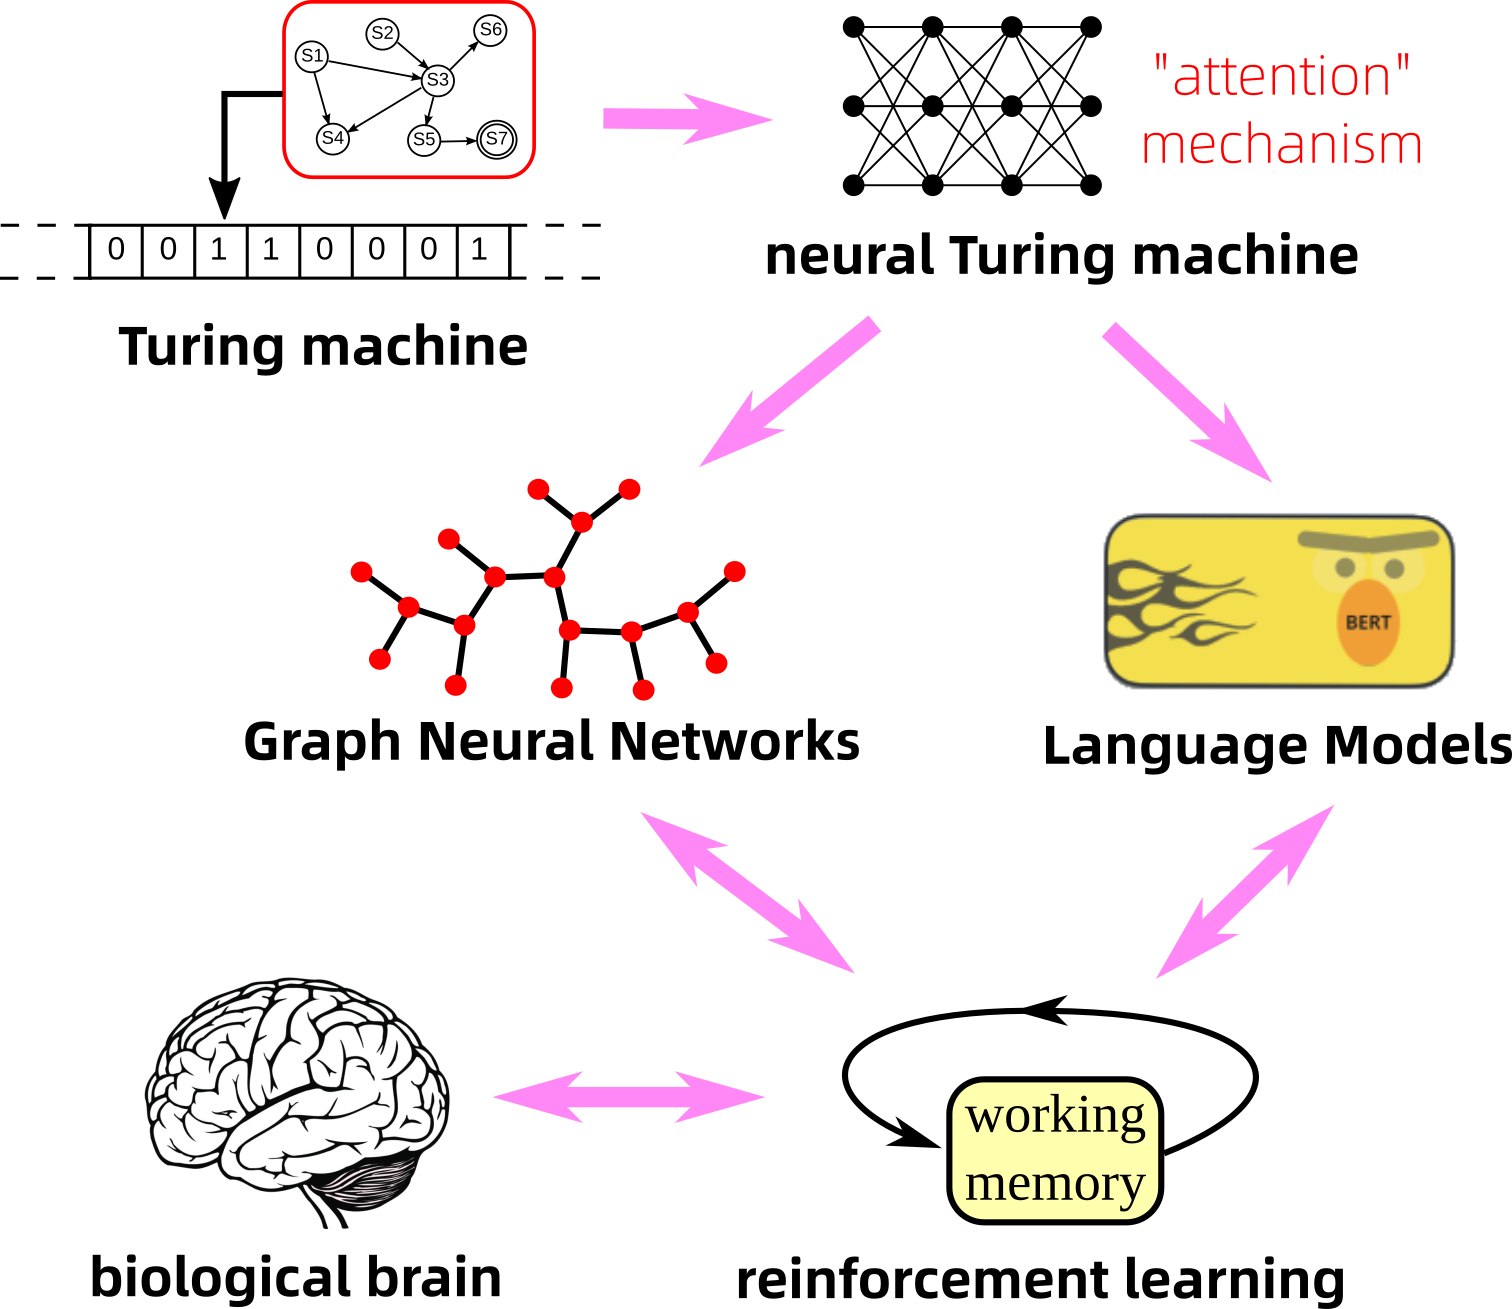
\includegraphics[scale=0.8]{AGI-standard-model.png}}}
\end{equation}
\cc{
然后关键的一步就是将 \textbf{end-to-end} 训练的模型 变成 \textbf{RL} 训练的形式\footnote{通常 RL 的 actions 是在环境中的动作,但我的 RL 模型 要求 actions 是一些 \textbf{思想} (thoughts),这并不规范,可能产生传统 RL 没有的问题。}。
前者可以看成是 进行 ``few-steps'' 的逻辑推导,而后者是可以 ``任意多步'' 的推导,而且这些推导 互相之间有 \textbf{协同效应} (一个推出来的结果帮助另一个新的推导)。 正是因为 \textbf{闭环训练} 容许了这些 协同效应,令 RL 系统有可能学习出能够\textbf{解释}世界的 logic theory.
}{
The next, crucial step is to change end-to-end training to the RL setting\footnote{Normally, actions in RL refer to what are performed in the external environment, but in my somewhat unorthodox formulation, actions are ``thoughts''.  This may create some problems not seen in traditional RL.}.
The former can be seen as allowing ``few-steps'' logic inference, whereas the latter allows \textbf{arbitrary number} of inference steps.  This enables logic rules to make use of results from other rules, creating a \textbf{cooperative effect}.  Precisely due to closed-loop training and the synergy, an RL agent may be able to learn a logic theory that \textbf{explains} the world.
}
\end{minipage}
\end{preview}

\begin{preview}
	
\setlength{\parskip}{0.4\baselineskip}
\begin{textblock*}{20cm}(2.1cm,2cm) % {block width} (coords) 
	{\color{red}{\large \textcircled{\small 3}}}
	\hspace{8cm}
	\color{blue}{\footnotesize 逻辑化 AGI 基础}
\end{textblock*}
\vspace*{0.3cm} 

\section{Neural Turing Machines and Transformers}

The \textbf{attention mechanism} was first proposed in the ``\textbf{Neural Turing Machine}''  paper by Graves \textit{et al} [2014].

Recall that a Turing machine is a \textbf{Finite State Machine} augmented with a \textbf{Memory Tape}:
\begin{equation}
\vcenter{\hbox{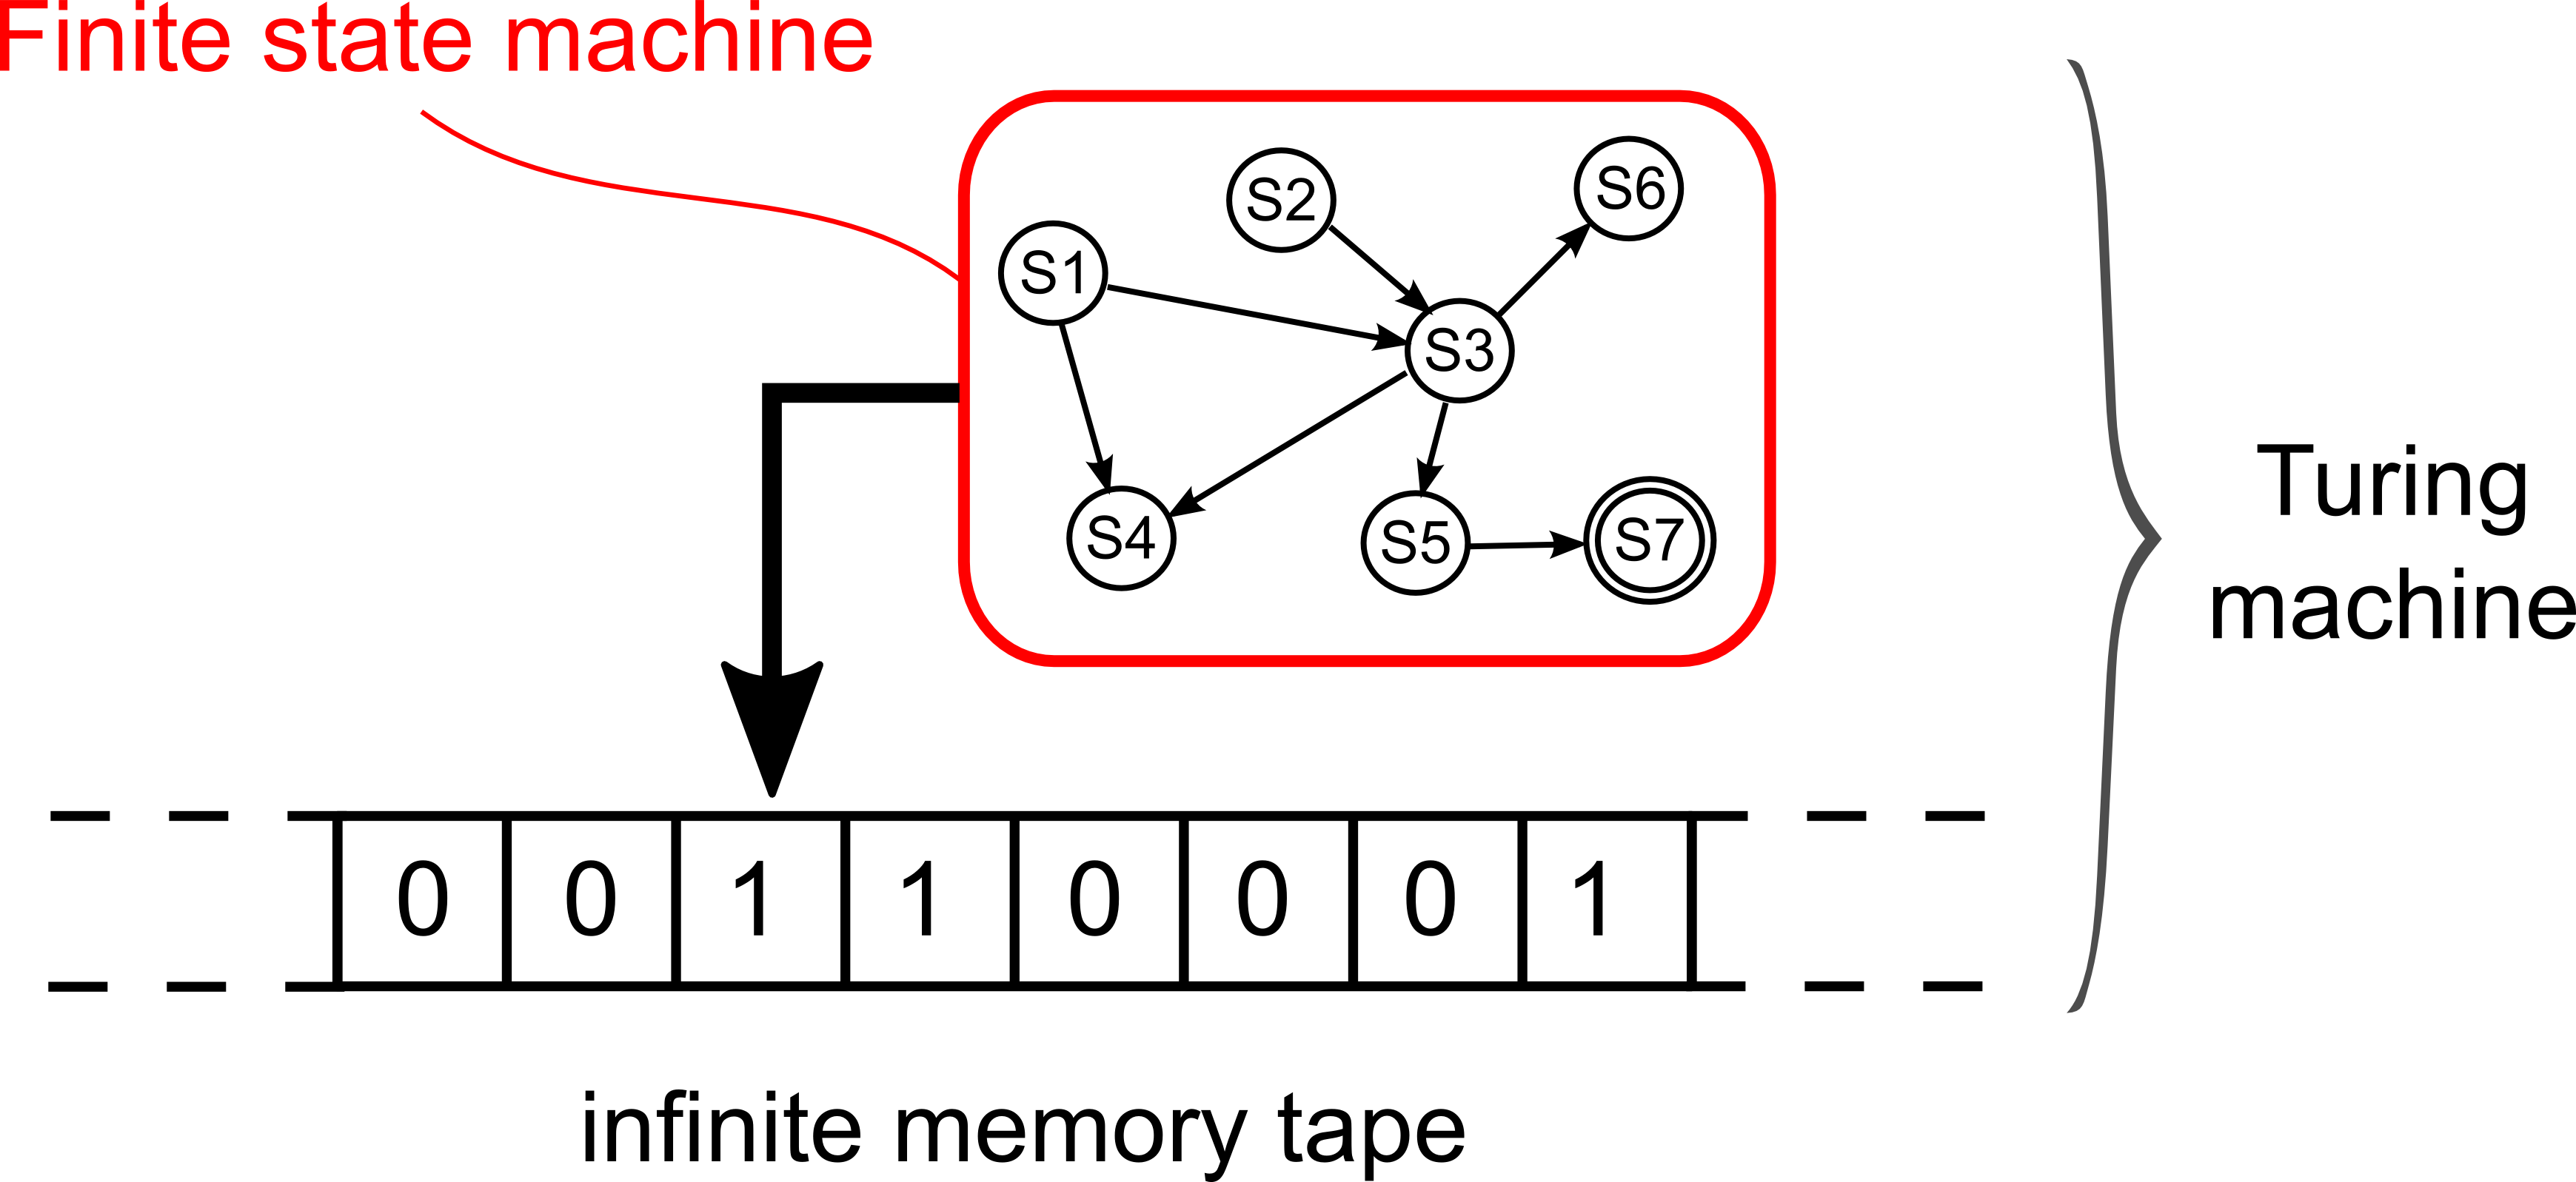
\includegraphics[scale=0.9]{Turing-machine.png}}}
\end{equation}

In Neural Turing Machines, Graves \textit{et al} proposed the attention mechanism for an RNN ``Controller'' (playing the role of the Finite State Machine) to read and write from a \textbf{Memory Matrix} (the tape), using a content-based addressing method.

The Memory Matrix $M$ consists of $N$ items, each of constant size.  \textit{The discreteness of the address would introduce discontinuities in gradients of the output}, hence we need an \textbf{Attention Vector} to focus on a specific location in the memory matrix $M$.

The Attention Vector $\vec{a}$ is calculated via the following formula, familiar to students of the Transformer: 
\begin{equation}
\vec{a} = \mathrm{soft} \max_i \{  \mathcal{D}(K, M_i) \}
\end{equation}
where $D()$ is a similarity measure between the key $K$ and memory item $M_i$.  The key $K$ is emitted by the Controller as the value that it is looking for.

This then evolved into the \textbf{Self Attention} mechanism used in all Transformers.  Now let us refresh with this diagram illustrating Self-Attention (redrawn from a blog article on the web):

\begin{equation}
\vcenter{\hbox{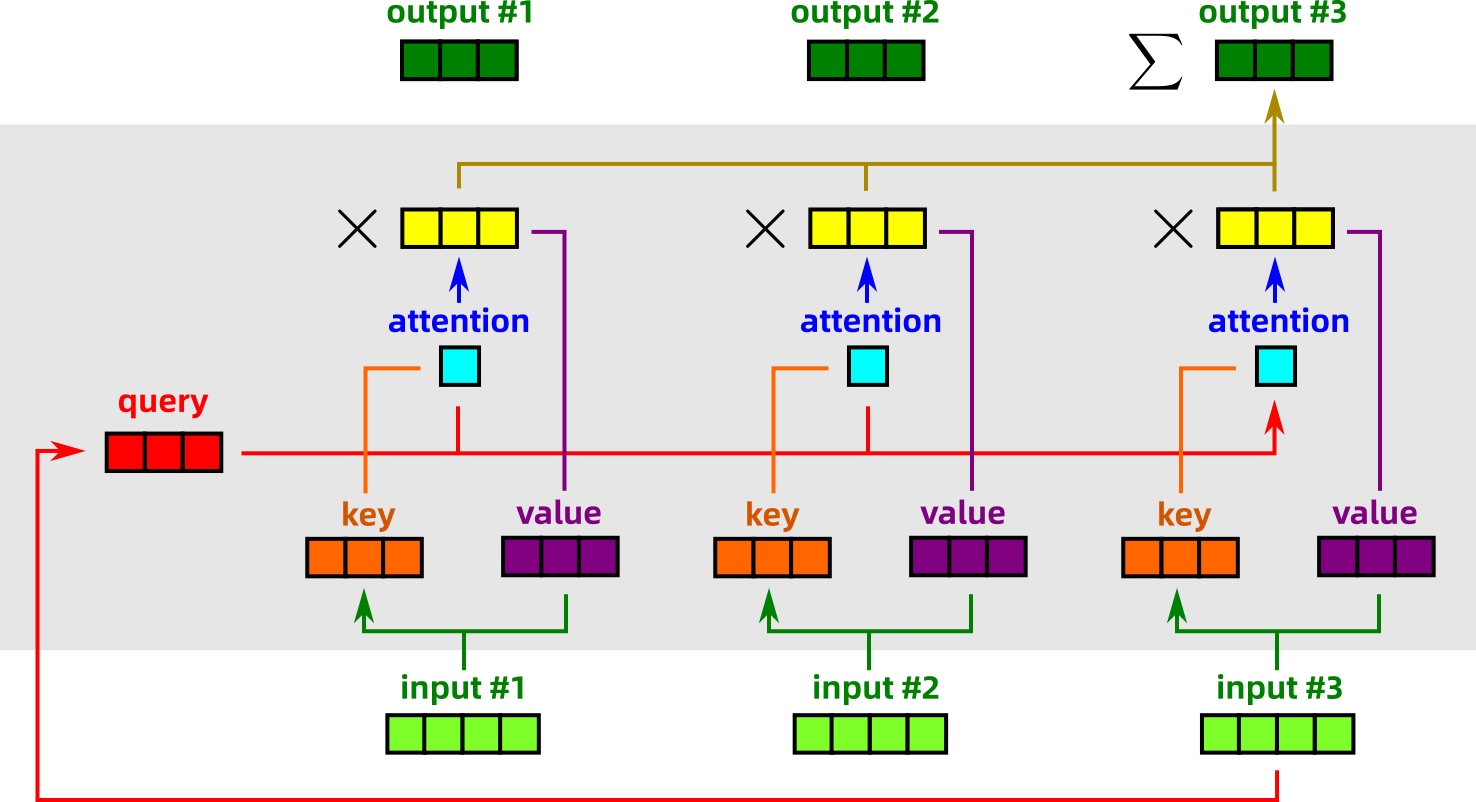
\includegraphics[scale=0.9]{self-attention-2.png}}}
\end{equation}

The research done by Olah \textit{et al}, in their 2021 paper \textit{\uline{A Mathematical Framework for Transformer Circuits}}, is very helpful towards understanding Transformers and Self-Attention.  

For example when we say ``all men are mortal'':
\begin{equation}
\forall x. \; \mbox{Human}(x) \Rightarrow \mbox{Mortal}(x)
\end{equation}
any object instantiated as $x$ (eg. ``Socrates'') would have to be \textbf{copied} from the LHS to the RHS.
\end{preview}

\begin{preview}
\setlength{\parskip}{0.4\baselineskip}
\begin{textblock*}{20cm}(2.1cm,2cm) % {block width} (coords) 
	{\color{red}{\large \textcircled{\small 4}}}
	\hspace{8cm}
	\color{blue}{\footnotesize 逻辑化 AGI 基础}
\end{textblock*}
\vspace*{0.3cm} 

\section{Abductive reasoning}
\label{sec:abductive-reasoning}

Abduction has been relatively neglected in AGI research, which had focused on forward inference.  Recently there is a call to study this important aspect.

In logic, abduction means finding the \textbf{explanation} for some known facts.  An explanation $E$ is simply some propositions that imply the known fact $F$, ie, $E \Rightarrow F$.

For example, why do we think a certain actress, say Marilyn Monroe, is ``sexy'' \footnote{I use this example because ``sexy'' is a kind of high-level concept and we apply this concept commonly when we meet other people.  Every one can relate to the ``reasons'' why we think someone is sexy.} ?  That's because we recognize she has some features (visual or otherwise, no need to enumerate them explicitly) that we consider sexy.  So, $E_1 \wedge E_2 \wedge .... \Rightarrow \mathrm{Sexy}$.  Those conditions \textbf{imply} she is sexy, and they are the \textbf{explanation} for her sexiness.

Why is abduction important?  For example, when a waitress says ``The Ham Sandwich left a big tip'', \textit{Ham Sandwich} here refers to the customer who ordered it (an example of metonymy).  The AI knows the plain facts such as that someone ordered a ham sandwich, and then it abduces that the most likely \textbf{interpretation} of the phrase ``Ham Sandwich'' is as the person associated with it.  This is the basis of \textbf{Abductive Interpretation of Natural Language} proposed by Jerry Hobbs:
\begin{equation}
\vcenter{\hbox{
\includegraphics[scale=0.7]{Jerry-Hobbs.png}}}
\end{equation}

So abductive reasoning is basically just \textbf{bidirectional} inference.

When a system has both forward and backward connections, it forms a loop and its dynamics is likely to produce ``\textbf{resonance}''.  This harks back to the ART (\textbf{Adaptive Resonance Theory}) proposed by Grossberg and Carpenter beginning in the 1980s.

Such resonance behavior can be viewed as the system seeking to minimize an energy, ie, trying to find the ``best explanation'' to a set of facts.  

This is also corroberated by neuroscientific evidence:  areas in the cerebral cortex are replete with both forward- as well as \textbf{back-projections}, as depicted in diagram (\ref{fig:cortex-back-projections}).  We can further abstract this with the following diagram, where $F$ and $G$ are not functions but \textbf{optimization constraints}:
\begin{equation}
\begin{tikzcd}
\vec{y} \arrow[d, bend left, "G"]  \\
\vec{x} \arrow[u, bend left, "F"]
\end{tikzcd}
\end{equation}
If the input $\vec{x}$ produces the output $\vec{y}$ after some iterations, then it is likely that the output $\vec{y}$ would produce $\vec{x}$ in the \textbf{inverse} direction.  In other words, we have a \textbf{neural} mechanism that implements a function $f$ and its inverse $f^{-1}$.  The significance of this (from the \textbf{learning} point of view) is that we only need to learn the function $f$ and we get $f^{-1}$ \textbf{for free}.

In logic, if forward inference is denoted as $\vdash_{\KBsymbol}$, where $\KBsymbol$ is a set of logic rules, then abduction is $(\vdash_{\KBsymbol})^{-1}$.  Abductive interpretation is basically a \textbf{constraint-satisfaction} process that uses inference rules in both directions.

\section{Dealing with assumptions}

\end{preview}
\end{document}
